% QUESTAO
Considere a função $f:A\longrightarrow B$ dada pelo diagrama. Determine $x$ quando $y=7$.

\parbox{0.3\linewidth}{

% ALTERNATIVAS
$x=5$
$x=3$
$x=4$
$x=6$
$x=2$

}\parbox{0.69\linewidth}{

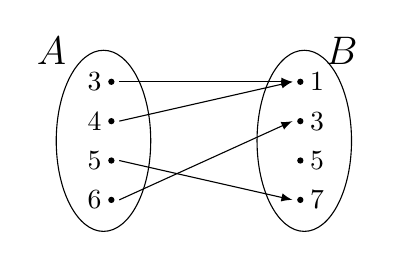
\begin{tikzpicture}[ >=latex, x=0.5cm, y=0.5cm ]

\draw[] (0,2.5) ellipse (1.2 and 2.3) node[above left] at (-0.7,4.2) {\Large$A$};

\fill (0.2,4) circle (0.4mm) node[left] {$3$};
\fill (0.2,3) circle (0.4mm) node[left] {$4$};
\fill (0.2,2) circle (0.4mm) node[left] {$5$};
\fill (0.2,1) circle (0.4mm) node[left] {$6$};


\draw[] (5.1,2.5) ellipse (1.2 and 2.3) node[above left] at (6.7,4.2) {\Large$B$};

\fill (5,4) circle (0.4mm) node[right] {$1$};
\fill (5,3) circle (0.4mm) node[right] {$3$};
\fill (5,2) circle (0.4mm) node[right] {$5$};
\fill (5,1) circle (0.4mm) node[right] {$7$};

\draw[->] (0.4,4) -- (4.8,4);
\draw[->] (0.4,3) -- (4.8,4);
\draw[->] (0.4,2) -- (4.8,1);
\draw[->] (0.4,1) -- (4.8,3);

\end{tikzpicture}

}

